\documentclass[a4paper]{article}
\usepackage{amsmath,amsfonts,amsthm}
\usepackage{fullpage}
\usepackage{float}
\usepackage{color}
\usepackage{graphicx}
\begin{document}

\newtheorem{lem}{Lemma}
\newtheorem{prop}{Proposition}
\newtheorem{rem}{Remark}
\newtheorem{thm}{Theorem}
\renewcommand{\a}{\mathbf{a}}
\renewcommand{\v}{\mathbf{v}}
\title{Multiscale Adaptive Representation of Signals}
\author{Cheng Tai}
\date{}
\maketitle
\abstract{}
\section{Overview of dictionary learning and wavelets}
It is now well acknowledged that sparse and overcomplete representations of data play a key role in many signal processing areas. The ability to represent a signal as a sparse linear combination of a few atoms from a possibly overcomplete dictionary lies in the heart of many applications of signal processing, examples include image/audio compression, denoising, and higher level tasks such as pattern recognition.

Over the years, many efforts have been put on designing dictionaries with certain properties. There are two lines towards this objective.  One line can be loosely called the analytic dictionary approach, which assumes the mathematical properties of the class of signals of interest, and develops optimal representations for that class of signals. Examples of this category include: Fourier basis, wavelets, wavelet tight frames\cite{daubechies2003framelets}, curvelets\cite{candes2000curvelets}, contourlets\cite{do2002contourlets}, etc. The other line takes a different route, it does not make any assumptions about the mathematical properties of the signals, instead it tries to learn the optimal dictionaries directly the data, examples of this category include: MOD\cite{engan1999method}, K-SVD\cite{aharon2006svd} and their variants, etc. Since the seminal work of Olshausen and Field\cite{olshausen1996emergence}, the field of dictionary learning has seen many promising advances. 


The different nature of the two approaches result in different implementation schemes. Models of the first kind are characterized by implicit transformations whereas models of the second kind has to explicitly apply the learned dictionary. But the major advantage of the second approach is that it leads to state-of-the art results in many low level signal processing applications. 

Despite the elegance and success of this methodology, there are some shortcomings that cannot be ignored especially when the models are plugged into applications, these include the following:
\begin{itemize}
\item computational cost is high. Assume the signal is of length $N$, the trained dictionary $A\in \mathbb{R}^{m\times N}$ is stored and used explicitly. Each multiplication of the form $Ax$ requires $O(mN)$ operations. In comparison, the analytic dictionary approach, such as the fast Fourier transform only takes $O(N\log N)$ operations, and the one level wavelet transform takes only $O(N)$ operations. The difference is huge. When dictionary learning models are plugged into applications, we have to solve a relatively complex sparse coding program, even with the fastest greedy algorithms, such as Matching Pursuit, the matrix multiplications still have to be carried out several times. Thus it is much less efficient compared to traditional transform methods.
\item restriction to low-dimensions. Because the learning procedure requires solving a relative complex non-convex optimization program, the signals that can be practically trained is restricted to have low dimensions, typically, $n\leq 1000$ is a reasonable limit. Partially because of this, in image processing applications, most popular models only train dictionaries on small image patches. An attempt to go beyond the limit raises a series of problems, including the need for an huge amount of training data and intolerable training time.
\item operating on a single scale. Dictionaries as obtained by the MOD and the K-SVD operate on signals at a single small scale. Past experience with wavelets has taught us that often times it is beneficial to process the signals at several scales, and operates on each scale separately. This issue is actually related to the previous ones, since the dictionary atoms that can be trained is small in size, which does not allow much room for multiple scales. There are some attempts in training multi-scale dictionaries, this direction has yet to be thoroughly explored.
\item Artifacts.  In low level tasks such as image compression, the dictionary learning approach operates in a patch by patch manner, which produces visually unpleasant block effects along the boarders of the patch,\cite{bryt2008compression}.  Post processing is often needed to remove these artifacts\cite{bryt2008improving}. 
\end{itemize}

A natural question is, is there any hope to get the best of both worlds? It is the goal of this paper to propose a partial solution to this question. In particular, we address two issues: the inefficiency of sparse coding used by most dictionary learning scheme to encode a new incoming signal and lack of a truly multi-scale representation. We will devise a novel representation of image signals, which is multi-scale in nature and is computationally efficient, and it is adapted to the signals as dictionary learning does. 

In particular, first we construct one layer adaptive wavelet tight frames. The wavelet tight frames are constructed in a manner that gives the sparest representations of the signals within all the admissible tight frames, we then use the one layer construction as a building block to construct multi-scale representations.
%\section{A First Attempt to Improve Computational Efficiency of Dictioanry Learning}
%There are two routes we can take to reach our goal. One starts from dictionary and the other from wavelet tight frames. A route which we will not detail but will ultimately lead us to the same goal is the following: start with image patches, instead of training unstructured dictionary, we train tight frames, this helps improving the computational efficiency in that we don't need to solve a sparse coding program any more, instead, just perform one matrix vector multiplications. Next, we make the dictionary convolutional, based on the premise that image patches are shift invariant at a certain scale. Then, we would reach at something similar to a one layer adaptive wavelet tight frame transform. 
\section{Single Scale Adaptive Wavelet Tight Frames}
We begin with a brief review of existing construction of wavelet tight frames.

\subsection{Wavelet Tight Frames}
In this subsection, we give a very brief introduction to wavelet tight frames, for a detailed introduction to this subject, the readers may refer to \cite{shen2010wavelet,daubechies2003framelets}.

Let $\mathcal{H}$ be a Hilbert space, we are mainly concerned with the case when $\mathcal{H}=L_p(\mathbb{R}^d)$. a system $X\subset H$ is called a tight frame if
\[
\|f\|_2^2 = \sum_{x\in X} |\langle f,x\rangle |^2, \quad \textrm{for any } f\in \mathcal{H}
\]
There are two operators that are associated with a tight frame, one is the analysis operator defined as
\[
W: f\in \mathcal{H} \rightarrow \{\langle x,f\rangle\}_{x\in X} \in l_2(\mathbb{N})
\]
and the other is the synthesis operator $W^T$, which is the adjoint operator of the analysis operator defined as
\[
W^T : \{a_n\} \in l_2(\mathbb{N}) \rightarrow \sum_{x\in X} a_n x\in \mathcal{H}.
\]
The system $X$ is called a tight frame if and only if $W^TW=I$, where $I: \mathcal{H} \rightarrow \mathcal{H}$ is the identity operator. In other words, given a tight frame $X$, we have the following canonical expansion:
\[
f=\sum_{x\in X} \langle x,f\rangle x, \quad \textrm{for any } f\in \mathcal{H}
\]
The sequence $Wf:=\{\langle f,x\rangle \}_{x\in X}$ are called the canonical tight frame coefficients. Thus, tight frames are often viewed as generalizations of orthonormal basis. In fact, a tight frame $X$ is an orthonormal basis for $\mathcal{H}$ if and only if $\|x\|=1,\forall x\in X$.

In signal processing applications, one widely used class of tight frames is the wavelet tight frames. The construction starts with a finite set of generators $\Psi:=\{\psi^1,\cdots,\psi^m\}$. Then consider the affine system defined by the shifts and dilations of the generators:
\[
X(\Psi)=\{M^{j/2}\psi^{l}(M^j\cdot -k),1\leq l\leq m, j,k\in\mathbb{Z}, M\in\mathbb{Z^+}\}.
\]
The affine system $X(\Psi)$ is called a wavelet tight frame if it is a tight frame satisfying
\[
f=\sum_{x\in X(\Psi)} \langle f,x\rangle x, \forall f \in \mathcal{H}.
\]
Wavelet tight frames used in practice are usually constructed from multi-resolution analysis(MRA). This is because a MRA structure is crucial for fast decomposition and reconstruction algorithms.  The MRA construction usually starts with a compactly supported scaling function $\phi$ with a refinement mask  $a_0$ satisfying
\[
\hat{\phi}(M\cdot)=\hat{a_0}\hat{\phi}.
\]
where $\hat{\phi}$ is the Fourier transform of $\phi$, and $\hat{a_0}$ is the discrete Fourier series defined as $\hat{a_0}(\omega):=\sum_{k\in\mathbb{Z}} a_0(k) e^{-ik\omega}$ and $\hat{a_0}(0)=1$. After obtaining the scaling function, the next step step is to find an appropriate set of filters $\{a_1,\cdots,a_m\}$ and define the set of functions called framelets $\Psi=\{\psi_1,\cdots,\psi_m\}$ by
\[
\hat{\psi_i}(M\cdot) = \hat{a_i}\hat{\phi},i=1,\cdots,m
\]
such that the affine system $X(\Psi)$ forms a wavelet tight frame. 

Given a filter $a\in l_2(\mathbb{Z})$, the discrete decomposition and reconstruction transform are defined in the following way. Define the one dimensional down-sampling and up-sampling operator:
\[
\begin{aligned}
	&[v\downarrow M](n):=v(Mn),\quad n\in \mathbb{Z}\\
	&[v\uparrow](Mn):=v(n), \quad n\in \mathbb{Z}
\end{aligned}
\]
where $M$ a positive integer denoting the down-sampling or up-sampling factor. Down-sampling and up-sampling operators in higher dimensions are carried out by performing one dimensional operators along each dimension. 

Define the linear convolution operator $S_a: l_2(\mathbb{Z}) \rightarrow l_2(\mathbb{Z})$ by 
\[
[S_a(v](n):=[a*v](n)=\sum_{k\in\mathbb{Z}} (a(-\cdot)*v \downarrow)M, \forall v\in l_2(\mathbb{Z})
\]
For a set of filters $\{a_i\}_{i=1}^m\subset l_2(\mathbb{Z})$, we define its analysis operator $W$ by 
\[
W=[S_{a_1(-\cdot)},S_{a_2(-\cdot)},\cdots,S_{a_m(-\cdot)}]^T.
\]
Its synthesis operator is defined as the transpose of $W$:
\[
W^T=[S_{a_1(\cdot)},S_{a_2(\cdot)},\cdots, S_{a_m(\cdot )}].
\]

It is natural to ask when the wavelet system $\Psi(X)$ forms a wavelet tight frame. Sufficient and necessary conditions are given by the so called Unitary Extension Principle(UEP). There are several versions of the unitary extension principles, in particular, we are interested in the one that is associated with discrete wavelet tight frames. For a survey of UEP, the reader may refer to \cite{benedetto2001wavelet}. The unitary extension principle states that:
\begin{thm}\cite{han2011adaptive}
Let $a_1,\cdots,a_m$ be finitely supported filters, the following are equivalent:
\begin{enumerate}
\item $W_a^T W_a = I$
\item for all $\omega \in [0,1)^d\cup M^{-1}\mathbb{Z}^d$,
\[
	\sum_{i=1}^m \hat{a_i}\overline{\hat{a_i}(\xi + 2\pi\omega})=\delta(\omega);
\]
\item for  all $k,\gamma \in \mathbb{Z}^d$,
\[
	\sum_{i=1}^m \sum_{n\in\mathbb{Z}^d} \overline{a_i(k+Mn+\gamma)}a_i(Mn+\gamma)=M^{-d}\delta(k).
\]
\end{enumerate}
\end{thm}
In particular, if the data are real numbers and no down-sampling is performed, then $W^TW=I$ is equivalent to 
\begin{equation}
\label{eq:uep}
\sum_{i=1}^m \sum_{n\in \mathbb{Z}^d} a_i(k+n) a_i(n)=\delta_k, \forall k\in \mathbb{Z}^d.
\end{equation}
The linear B-spline wavelet tight frame used in many image restoration tasks is constructed via the UEP. Its associated tree filters are :
\[
a_1=\frac{1}{4}(1,2,1)^T; \quad a_2=\frac{\sqrt{2}}{4}(1,0,-1)^T; \quad a_3=\frac{1}{4}(-1,2,-1)^T.
\]
Once the 1D filter $\{a_i\}_{i=1}^m$ for generating a tight frame for $l_2(\mathbb{Z})$ is constructed, the traditional way of generating higher dimensional tight frames is to use tensor products of 1D filters.

\subsection{Adaptive Construction}
The aforementioned wavelet tight frame is a shift-invariant system. We use shift-invariant systems because we accept the premise that at some proper scales, the statistical properties of image patches are translational invariant. Let $W_a$ be the matrix form of the analysis operator generated by the filters $\{a_i\}_{i=1}^m$, and let $W^T_a$ be the matrix form of the synthesis operator. Define $\mathcal{C}$ to be the set of filters that satisfy the full UEP condition, that is $\mathcal{C}=\{ \{a_i\}_{i=1}^m : W_a^TW_a=I\}$. We also consider the set of filters that approximately satisfy the full UEP condition within error $\delta$, $\mathcal{C}_\delta = \{\{a_i\}_{i=1}^m : \|W_a^TW_a -I\|_*\leq \delta\}$, where $\| \cdot \|_*$ means the operator norm, as in some image processing applications,  a small loss of information is acceptable.

For a specific class of images at hand, there are infinitely many discrete wavelet tight frames to choose from. Although they all provide perfect reconstruction of the input signal, some of them may provide sparser representations than the rest. It is natural to seek the filters that provide the sparest representation. That is, we look for the minimizer of the following optimization program:
\begin{equation}
\begin{aligned}
	&\min_{a_1,\cdots,a_m} \sum_{i=1}^m\Phi(v_i) \\
	\textrm{subject to} \quad&v_i = a_i(-\cdot)*x,\quad i=1,\cdots,m\\
	 & \{a_i\}_{i=1}^m \in \mathcal{C} \\
\end{aligned}
\end{equation}
where $\Phi(v_i)$ is a sparsity inducing function, it can be chosen as, for example, the $l_1$ norm or $l_0$ "norm" or the Huber loss. In our experiments, using different sparsity inducing terms does not seem to have much influence on the results, $l_1$ norm is slightly better in image restoration tasks. Hence we use $l_1$ norm in the following exclusively, this leads to:

\begin{equation}
\label{model:m0}
\begin{aligned}
	&\min_{a_1,\cdots,a_m} \sum_{i=1}^m \|v_i\|_1 \\
	\textrm{subject to} \quad&v_i = a_i(-\cdot)*x,\quad i=1,\cdots,m\\
	 & \{a_i\}_{i=1}^m \in \mathcal{C} \\
\end{aligned}
\end{equation}
In some image processing tasks, such as pattern recognition, a small deviation from the perfect reconstruction filters is acceptable. In that case, we consider
\begin{equation}
\label{model:m1}
\begin{aligned}
	&\min_{a_1,\cdots,a_m} \sum_{i=1}^m \|v_i\|_1 \\
	\textrm{subject to} \quad&v_i = a_i(-\cdot)*x,\quad i=1,\cdots,m\\
	 & \{a_i\}_{i=1}^m \in \mathcal{C_\delta} \\
\end{aligned}
\end{equation}



Let us have a look at what challenges the constraint pose to the numerical optimization. For simplicity, consider the case when the signals and the filters are one dimensional, each filter has support length $r$. We define a non-standard notation $Tr(M,k)$ for a real symmetric matrix $M$ to be the sum of entries along the $k$-th diagonal. In particular, $Tr(M,0)$ is the usual trace of a matrix.
Define the matrix  $A:=[a_1,\cdots,a_m]$. Then the constraint $ \{a_i\}_{i=1}^m \in \mathcal{C}$ is equivalent to 
\[
Tr(AA^T,k)=\delta_k, k=0,\cdots,r-1.
\]
For example, if there are $r$ filters and they are orthogonal to each other with $\|a_i\|=1/\sqrt{r}$, then the constraint is obviously satisfied. But in general, this algebraic constraint is difficult to deal with. 

Because of this algebraic constraint, this optimization program is not convex and a local minimum is all we can hope at best. Yet, past experience in machine learning tells us that a local minimum is oftentimes good enough to provide meaningful results, such is the case in our model.

The difference of \eqref{model:m0} and \eqref{model:m1} largely lies in the easiness of numerical computation. For \eqref{model:m0}, the constraint is exact, and we need to solve a sequence of unconstrained programs as is done with interior-point method or split-bregman algorithm. While for \eqref{model:m1}, we can get an approximate solution using the  following penalty method. 
\[
\begin{aligned}
	&\min_{a_1,\cdots,a_m} \sum_{i=1}^m \|v_i\|_1 + \eta \sum_k (Tr(A^TA,k)-\delta_k)^2 \\
	\textrm{subject to} \quad &v_i = a_i(-\cdot)*x,\quad i=1,\cdots,m
\end{aligned}
\]
where $\eta$ depends on $\delta$.
%\begin{prop}
%Let $\{a\}_{i=1}^m$ be the minimizer of \eqref{model:m0}, let $\{\hat{a}_i\}_{i=1}^m$ be the solution to the following program:
%\begin{equation}
%	\label{model:m2}
%	\begin{aligned}
%		&\min_{a_1,\cdots,a_m} \sum_{i=1}^m \|v_i\|_1 + \eta \sum_k (Tr(A^TA,k)-\delta_k)^2 \\
%		\textrm{subject to} \quad &v_i = a_i(-\cdot)*x,\quad i=1,\cdots,m
%	\end{aligned}
%\end{equation}
%Then, for sufficient large $\eta$, we can correct $\hat{a}$ to be a solution $a^*$ such that the infeasibility of $a^* \sim \mathcal{O}(1/\lambda^2)$ and $\|v^*\|_1 \leq \|v\|_1 + \mathcal{O}(1/\lambda)$.
%\end{prop}
%\begin{proof}
%	For notation simplicity, concatenate $\{a\}_{i=1}^m$ to form a single vector $a$, and similarly for $\{\hat{a}\}_{i=1}^m$. Let $F(a):=\sum_{i}^{m} \|a_j(-\cdot)*x\|_1$ and $G(a):= \sum_k (Tr(A^TA,k)-\delta_k)^2 $. 
%	As $\hat{a}$ is minimizer of \eqref{model:m2}, $ F(a)+\eta G(a) \geq F(\hat{a}) + \eta G(\hat{a})$. But $G(a)=0, G(\hat{a})\geq 0$, hence $F(\hat{a})\leq F(a)$ and $G(\hat{a}) \leq \frac{1}{\eta} (F(a)-F(\hat{a}))$. Since $F(a)$ is bounded, $G(\hat{a}) \sim \mathcal{O}(1/\eta)$ as $\eta\rightarrow\infty$. Now we have a solution $\hat{a}$ with infeasibility $\mathcal{O}(1/\eta)$. we correct it as follows: for sufficient large $\eta$, $G(\hat{a}+e)=G(\hat{a})+\nabla G(\hat{a})e + o(\|e\|_2)$. As $G(a)$ is continuously differentiable, let $G(\hat{a})+\nabla G(\hat{a})e =0$, we have $e=-(\nabla G(\hat{a}))^{\dagger} G(\hat{a})$ where the $\dagger$ means Moore-Penrose Pseudo inverse, which gives a solution to the linear equation with smallest $l_2$ norm. Let $\sigma_m$ be the smallest singular value of $\nabla G(\hat{a})$, then because of our choice of $e$, we have $\|e\|_2 \sim \mathcal{O}(\frac{1}{\sigma_m \eta})$ and $G(\hat{a}+e)\sim \mathcal{O}(1/\eta^2)$. Define $a^*=\hat{a}+e$. Therefore, $\|v^*\|_1 - \|v\|_1 =\sum_{j=1}^m (\|a^*_j(-\cdot)*x\|-\|a_j(-\cdot)*x\|_1\leq \sum_{j=1}^m (\|a^*_j(-\cdot)*x\|-\|\hat{a}_j(-\cdot)*x\|_1\leq Cm\|e\|_1\leq C\sqrt{mr}\|e\|_2\leq C\frac{\sqrt{mr}}{\sigma_m\eta}$.
%	
%		\end{proof}

%\begin{rem}
%	For the sole purpose of getting nearly perfect reconstruction filters, the second term in the above model can be replaced by the following sample reconstruction error:
%\begin{equation}
%	\begin{aligned}
%		&\min_{a_1,\cdots,a_m} \sum_{i=1}^m \|v_i\|_1 + \eta \|y-\sum_i a_i*a_i(-\cdot)*y\|_2 \\
%		\textrm{subject to} \quad &v_i = a_i(-\cdot)*x,\quad i=1,\cdots,m
%	\end{aligned}
%\end{equation}
%where $y$ is a sufficient large signal with each entry sampled from, e.g., a normal distribution.
%\end{rem}
%Optimization program \eqref{model:m2} is relatively easier to solve, we call it the sampling version of model \eqref{model:m1}. In practice, $\eta$ is chosen based on our tolerance of deviation from perfection reconstruction filters. By letting $\eta$ goes to $\infty$, we recover \eqref{model:m1}.  An illustration of the filters obtained is shown in Figure 1.



So far, the models are based on the premise that the signals can be written as a sparse linear combination of translational invariant wavelets. In practical applications, there may be perturbations or noises added to the coefficients, it is better to consider the following variant of model \eqref{model:m1} which allows small perturbations of the coefficients.

An illustration of the filtered obtained is in Figure \ref{fig:1}.
\begin{equation}
\label{model:m3}
\begin{aligned}
	&\min_{a_1,\cdots,a_m,v_1,\cdots,v_m} \sum_{i=1}^m \|v_i\|_1  + \lambda \sum_{i=1}^m \|v_i - a_i(-\cdot)*x\|_2^2\\
	\textrm{subject to} \quad& \{a_i\}_{i=1}^m \in \mathcal{C_\delta} \\		 
\end{aligned}
\end{equation}

This program can be solved, for example, by the interior-point method. But it is slow in general. A better solution for $l_1$ optimization program is the split Bregman method\cite{goldstein2009split}. The details are given in the appendix.

\begin{figure}[h!]
    \centering
    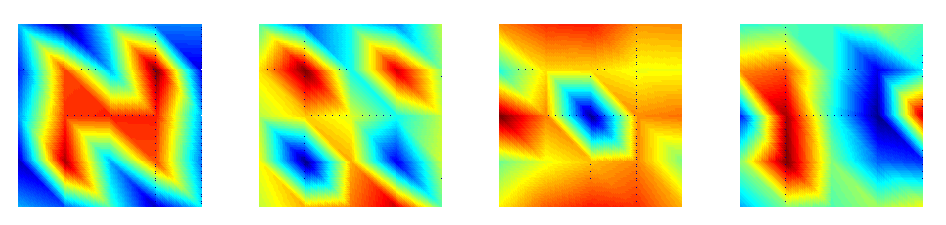
\includegraphics[width=0.5\textwidth]{fig11.eps}
  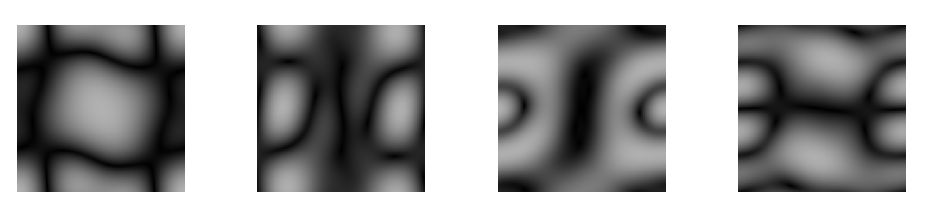
\includegraphics[width=0.5\textwidth]{fig12.eps}
    \caption{An example of learned filters and their Fourier spectrum.}
    \label{fig:1}
\end{figure}
Another key feature of this variant  is that unlike the previous model, the wavelet coefficients $\{v_i\}$ is no longer linearly dependent on $x$ given the filters $\{a_i\}_{i=1}^m$. Yet the coefficients can still be computed efficiently. Indeed, given the learned filters $\{a_i\}_{i=1}^m$ and the new input signal $x$, the coefficients are obtained by 
\[
\min_{v_1,\cdots,v_m} \sum_{i=1}^m \|v_i\|_1 + \lambda \sum_{i=1}^m \|v_i - a_i(-\cdot)*x\|_2^2,
\]
the solution of which is given explicitly:
\[
v_i = \mathcal{T}_{1/2\lambda}( a_i(-\cdot)*x),\quad i=1,\cdots,m
\]
where $\mathcal{T}: \mathbb{R}\mapsto \mathbb{R}$ is the soft-thresholding operator defined by
\[
\mathcal{T}_a(x)=\left\{ \begin{array}{lr}  (|x|-a)sign(x), &\textrm{ if } |x| > a \\0, &\textrm{otherwise}\end{array}\right . .
\]
When $\mathcal{T}$ operates on a vector, it operates on each component of the vector.


A special case of this variant, when the support of $a_i$ is of size $r\times r$ and $m=r^2$ and the filters are orthogonal to each other is proposed independently in \cite{cai2014data}, and local solution is found by iteratively solving the $\{v_i\}_{i=1}^m$ and $\{a_i\}_{i=1}^m$.

To this end, we have introduced the construction of adaptive wavelet tight frames for one layer. When plugged into applications, the results produced are comparable to those obtained by the dictionary learning paradigm, some numerical illustrations are given in section 5. In addition, we observed a quite unexpected and intriguing phenomena that we would like to share with the readers.

\subsection{An Intriguing Phenomenon}
\textbf{A unique low frequency filter}. The most commonly used wavelets and wavelet tight frames constructed using MRA has only one low frequency filter by design. As a result, it enables a fast multi-level decomposition and reconstruction algorithms, to get a multi-level representation of the signal, we successively apply the same filters to the coefficients representing the low frequency information. This structure is illustrated in Figure 2a. On the other hand, as one can notice, the UEP does not distinguish between low frequency and high frequency filters, all the filters jointly satisfy an algebraic constraint. From this perspective, indeed, one can use multiple low frequency filter. The cost of doing so is increased computational cost, represented by multiple branching point in the tree diagram. So for the algorithm to be of practical use, especially when computational efficiency is a concern, it is better to maintain a unique low frequency filter. Taking this into consideration, one is attempted to add the following linear constraints to the previous model:
\begin{equation}
\label{eq:low}
\sum_{i\in\mathbb{Z}^2} a_1(i)=1,\quad \sum_{i\in \mathbb{Z}^2} a_k(i)=0, k\in\{2,\cdots,m\}
\end{equation}
And if the above constraint is not incorporated, one would expect the resulting filters would be of diverse frequencies.

Surprisingly, we found that, on many datasets, the filters learned contains exactly one low frequency filter even without the above constraint. That is, constraint \eqref{eq:low} is automatically satisfied!  Numerically, what this means is that when the filters are normalized to have unit $l_2$ norm, then $ |\sum_{i\in \mathbb{Z}^2} a_k(i)| < 10^{-4}, k\in\{2,\cdots,m\}$. This phenomenon is stable regardless of the number and support size of the filters. We observed this phenomenon on many datasets, including the Yale-face dataset, the Caltech-101 dataset, the Fingerprint dataset, and a large number of randomly chosen natural photos. However, this phenomenon is not entirely universal, we observed multiple low frequency filters on the dataset Mnist. Apparently, this phenomenon has to do with the characteristics of the particular class of images and reflects the structure of the function space of all "natural images" to some extent. A natural question is: for what class of signals, can we observe such a phenomenon?

This phenomenon is assuring in that the filters produced by \eqref{model:m1} now has exactly the same form as the familiar wavelets and wavelet tight frames, hence can be used in the same way without any further troubles. 

On the other hand, since this phenomenon is ubiquitous for natural photos, it tells us some partial information about the structure of the space of all "natural images", which traditional wavelets are known to compress very well. The coincidence that manually designed wavelet happen to agree with the adaptively learned filters with sparsity in mind partially explains the successful applications of compressing natural images using wavelets in the past two decades.

From a practical point of view, one can always first try to solve \eqref{model:m1} without the low frequency constraint, and see if there happen to be a unique low frequency filter, if so, then there is a good chance that one can replace the wavelets or wavelet tight frames with adaptive versions at no additional cost. If not, one may consider incorporating the constraint explicitly.

\subsection{Recover Predefined Wavelets}
As the proposed model is an adaptive version of the wavelet tight frame, it would be natural to ask when could we recover the wavelet filters. Numerically, we observe that if the signals are indeed generated using sparse linear combinations of the predefined wavelets, then the learned filters automatically recover the predefined wavelet filters. This is related to the exact recover problem in dictionary learning. There, the problem is suppose the data matrix $X$ is generated by linear combination of dictionary atoms $X=DC+\epsilon$, then ask under what conditions can we recover $D$ and $C$ simultaneously given the observations $X$? See [][] for two recent results in direction. In our case, the dictionary is of special form and cannot be explained by the results there.

In the numerical experiment, we generate the signals of Daubechies wavelets with different level of sparsity and learn the filters by solving \eqref{model:m1}. Measure of success is the wavelet filters are exactly recovered( within error $10^{-5}$), repeat each setting multiple times and record the ratio of success in the following table:
\begin{center}
\begin{tabular}{| c | c | c | c| c | c |}
\hline
Density & db2\_32 & db2\_64 & db3\_64 & db12\_64 & db24\_64 \\
\hline
0.1 & 1 & 1 & 1 & 1 & 1 \\
\hline
0.2 & 1 & 1& 1 & 1 & 1 \\
\hline 
0.3 & 1 & 1 & 1 & 1 & 1  \\
\hline
0.4 & 1 & 1 & 1 & 0 & 0  \\
\hline 
0.5 & 0 & 0 & 0 & 0 & 0 \\
\hline
\end{tabular}
\end{center}
We note that if the signals indeed have a sparse representation in the wavelet domain, then the algorithm can successfully recover the wavelet filter. Above some threshold, however, the algorithm fails to recover the wavelet filters catastrophically. This is not surprising, after all the signals are no longer sparse in the wavelet domain. It's interesting to that there seems to be a phase transition between the success and failure regions.


\section{Extension to Mulitple Layers}
\subsection{Three Structures}
In this section, we extend the previous construction of adaptive wavelet tight frames to multiple layers. Going from one layer to multiple layers, we consider three typical structures illustrated in the following Figure.
\begin{center}
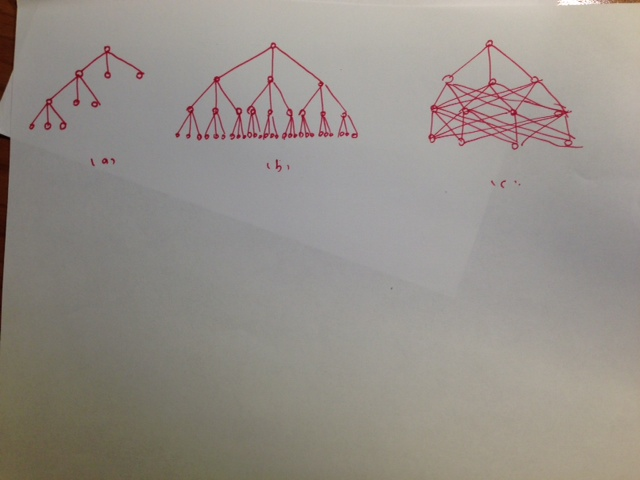
\includegraphics[scale=0.4]{arch.jpg}
\end{center}

The first structure is a $m$-ary tree which has at most one brunching point at each depth. This corresponds to the multi-level fast wavelet or wavelet tight frame transform. The root node represents the input image, (for illustration purpose, the input image has only one channel), applying $m$ filters on the input, we get $m$ sets of wavelet tight frame coefficients. Each set of coefficients is represented using $m$ child nodes. The left most node always represents the low frequency coefficients. To do multi-level transform, we successively apply the same filters on the low frequency coefficients. Thus, for a level $L$ wavelet tight frame transform, the structure we get a tree of depth $L+1$ . 

This structure arises naturally in wavelet tight frames generated using MRA. The major advantage is the efficient decomposition and reconstruction algorithm. For level-$L$ transform with downsampling, it takes only $\mathcal O(mN)$ operations for the decomposition of a signal of length $N$. To apply structure, the existence of a single low frequency filter is assumed. We can extend the previous one layer construction to this structure if there happen to be one low frequency filter or is constrained to have only one low frequency filter.  This structure is mostly useful in image compression tasks, and the coefficients are critically down-sampled.

The second structure is a full $m$-ary tree. Compared with the first architecture, instead of doing transforms on the low frequency coefficients only,  transforms are performed on the coefficients.  Apparently, the computational cost is now much larger. It is not appropriate for image compression or restoration tasks, but good for classification. Adaptation of the one layer model to this structure is straight forward. As the computational cost grows exponentially with the number of layers, we have to implement this structure with care and possibly some tricks in practice.  Examples of this structure include the scattering transform proposed by Mallat et.al. \\

The third structure resembles the convolutional neural networks. The first layer is still the same as the previous two, below that, the tree structure is replaced by a  locally connected  structure. This structure is more elaborate and requires some explanation which we give in the next subsection.

\subsection{The Proposed Multi-scale Structure}
The architecture consists an input layer and a few intermediate layers. The first layer is the same as the previous two structures. The intermediate layer accepts as input a few sets of coefficients produced by the previous layer, and produces another sets of output coefficients, not necessarily of the same size as the input. The input and output can be thought of as multi-channel images. The goal of the layer is still to produce sparse approximations of the input. Let $\{x_1,\cdots,x_m\}$ be the input coefficients, $\{v_1,\cdots,v_n\}$ be the output coefficients. The decomposition is defined as:
\begin{equation}
v_j = \sum_i a_{ij}(-\cdot)*x_i,\quad j=1,\cdots,n
\end{equation}
and the reconstruction is defined as 
\begin{equation}
x_i = \sum_j a_{ij}*v_j, \quad i=1,\cdots, m.
\end{equation}
The objective is to learn $\{a_{ij}\}, i\in \{1,\cdots,m\}, j\in \{1,\cdots, n\}$ which gives the sparest representation within the class of perfection reconstruction filters. Recognizing this as a 3D convolution, the UEP condition without downsampling then reads:
\begin{equation}
\label{uep:3d}
\sum_{i=1}^m\sum_{j=1}^n  \sum_{n\in \mathbb{Z}^3} a_{ij}(k+n)a_{ij}(n) = \delta(k).
\end{equation}

We could explicitly incorporate this constraint and repeat what did in the previous sections. This amounts to solving
\begin{equation}
\begin{aligned}
	&\min_{ \{a_{ij}\} } \sum_j \|v_j\|_1 \\
	\textrm{subject to} &\quad v_j = \sum_i a_{ij}(-\cdot)*x_i \\
		&\{a_{ij}\} \textrm{ satisfies \eqref{uep:3d}} \\
\end{aligned}
\end{equation}
On the other hand, we could solve a sampled approximation of the UEP constraint as
\begin{equation}
\label{eq:m3}
\begin{aligned}
\min_{a_1,\cdots,a_m, v_1,\cdots,v_m}& \sum_j \|v_j\|_1 \\
 \textrm{s.t.}  \quad v_j& = \sum_{i} a_{ij}(-\cdot)*x_i \\
	u_j&=\uparrow\downarrow(\sum_i a_{ij}(-\cdot)*y_i), \forall j. \\
	&\sum_i \|y_i - \sum_j a_{ij}*u_j\|_2 \leq \delta 
\end{aligned}
\end{equation}

where $y$ is randomly sampled vectors of sufficient size, and the $\uparrow \downarrow$ represented a down-sampling followed by a up-sampling operation. It could be omitted if we are only interested in un-decimated wavelet tight frames. The sampling operator need not be linear, it could be, for example max pooling and it reverse which are defined as 
\[
\downarrow(c_1,\cdots,c_n) = (\arg\max_{c_1,\cdots,c_n} |c_i|, \arg\max_{i=1,\cdots,n} |c_i|)
\]
and its reverse
\[
\uparrow(v,p)=(0,0,v[p],\cdots,0) \textrm{ with $v$ at the $p$-th location}.
\]
This is particularly useful for classification tasks.Unlike the linear sampling, in this case, we have to record both the value and position to get a natural reverse operation.

Similar to what we did before, in the case where there is perturbation on the coefficients, we consider the following variant which we use in the numerical experiments.
\begin{equation}
\label{eq:m5}
\begin{aligned}
\min_{\{a_{ij}\}, v_1,\cdots,v_m}& \sum_j \|v_j\|_1 + \lambda \sum_j \|v_j-  \sum_{i} a_{ij}(-\cdot)*x_i \|_2^2\\
 \textrm{s.t.}  	\quad 	u_j&=\uparrow\downarrow(\sum_i a_{ij}(-\cdot)*y_i), \forall j.\\
&\sum_i \|y_i - \sum_j a_{ij}*u_j\|_2  \leq \delta\\
\end{aligned}
\end{equation}
There is a subtlety considering stacking intermediate layer to form a multi-scale structures. That is, the output to input relation cannot be linear, otherwise stacking multiple layers would just be equivalent as a one layer structure. The non-linearity in our model may possibly come from two sources: one is the nonlinear sampling procedure, the other is the thresholding in the encoding stage.

Using \eqref{eq:m5} as a building block, we stack multiple layers together, we finally get the multi-scale structure depicted in Figure 2. The filters are all learned in a  layer by layer fashion, starting with the first one. Once the optimization has converged for the layer, we then move on to learn the next while keeping all filters in previous layers fixed. 

\section{Numerical Illustrations}
In this section, we provide examples for the possible applications of the representation developed in the previous sections. Examples in image compression, denoising, classification will be given. 
\subsection{Image Compression}
The models discussed so far is merely a view point. The only way to tell if these models work in reality is to apply them. We consider in this subsection the problem of image compression. Compression using adaptive wavelet tight frames that induces sparsity seems to be a very natural approach. Nevertheless, developing a mature compression scheme that competes favorably with JPEG2000 is very hard, as in this method, the entropy coding stage has been perfected. It is not sufficient to provide only the representation stage, one must provide appealing entropy coding as well. Still, we can address a specific coding task, where the entropy coding stage becomes secondary. 

When we consider a narrow and specific class of images, the amount of redundancy increases, hence enabling a better compression performance, for this reason, we consider the fingerprint image dataset. Such image class is what wavelets became known for and is also important application wise.

We compare two elementary compression schemes, one is predefined wavelet tight frames generated from Daubechies wavelets, db3, the other is the adaptive wavelet tight frame proposed in [], which has $4$ filters of size $6\times 6$ and is trained on the fingerprint dataset [].  Hence adaptive wavelet tight frame and the predefined wavelet tight frame has the same support size and the same total number of filters.  Given a tight frame and an image, we perform a 7-level transform, and keep only a fixed fraction of the largest coefficients in absolute value. The proportion of kept coefficients ranges from $1/2$ to $1/20$. Those coefficients are then used to reconstruct the image. We use PSNR(peak signal to noise ratio) to measure the quality of the compressed image. The result is shown in Figure \ref{fig:3}
\begin{figure}[h!]
    \centering
    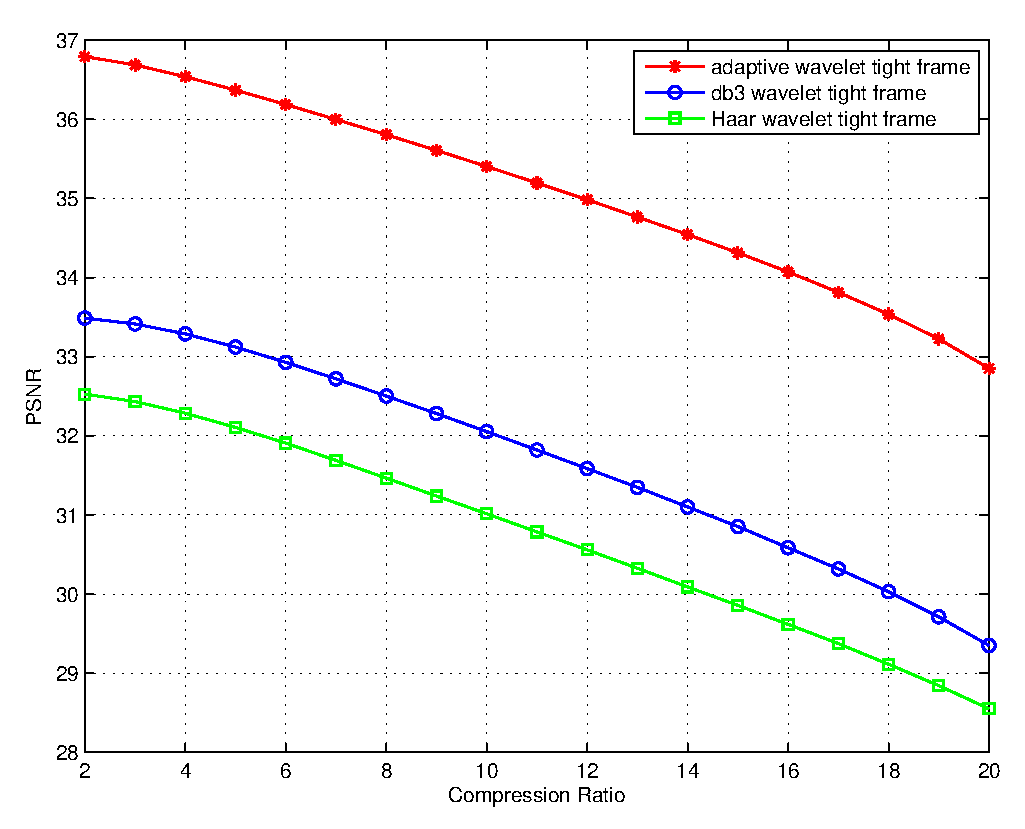
\includegraphics[width=0.4\textwidth]{figure51.eps}
    \caption{image compression illustration}
    \label{fig:3}
\end{figure}
The figures indicates the adaptively constructed tight frames is more effective in compressing the images. Training adaptive wavelet frames is also possible from a single image.
\subsection{Image Denoising Examples}
Images often contain noise, which may due to sensor imperfection, pool illumination, etc. Removing such noise is of benefit in many applications. Being perhaps the simplest possible inverse problem, it provides a convenient platform over which image processing ideas and techniques can be tested. Numerous contributions in the past few decades address this problem from many diverse point of view. The simplest of which is perhaps the wavelet domain thresholding.  It was originally proposed in [], later more sophisticated methods are developed and showed better performance such as the nonlocal means, BM3D, and the more recent ones based on dictionary learning ideas. 

We have no intention of providing a survey of this vast activity on image denoising in this subsection. Instead, for the same illustration purpose, we demonstrate the results of applying adaptive wavelet tight frames to this problem and compare it with a specific model of interest, the K-SVD model. As it is closely related to the proposed model and is shown to achieve state of the art results.

We assume the image is corrupted by some additive noise. That is 
\[
g=f+n
\]
where $f$ is the clean image, $g$ is our observation, and $n$ is the noise with unknown distribution.The algorithm using adaptive wavelet tight frames is the following: let $W$ be the decomposition operator associated with the wavelet tight frame, given a noisy image $g$, choose a scalar $\lambda$, then the denoised image is
\[
\hat{g} :=W^T \mathcal{T}_{\lambda} (Wg)
\]
where $\mathcal{T}$ is the soft thresholding operator introduced in section []. $\lambda$ obviously depends on the noise level, but since we have no prior knowledge of the noise distribution, this value can only be chosen by experiments.Unlike image compression, in image denoising applications, we can afford using very redundant systems. The extra redundancy is proven to yield to produce better results than the critically sampled wavelet frames in practice. Therefore, we use relatively redundant systems in the three examples below.

In this first example, the input is single image normalized to $[0,1]$ and is corrupted with additive gaussian noise with $\sigma=0.1$. We train the filters both from the noisy image and clean image. The filter is of support size $6\times 6$ and we train $36$ of them .The result is in Figure [].  The PSNR shown is selected by grid search to produce best PSNR. It is not surprising that the filters learned from a clean image produces better quality image. The performance of K-SVD algorithms depends on the number and size of the atoms in the dictionary. Generally, the performance increases as we increase the number of atoms as long as the number is not too large. In this example, $256$ atoms with size $6\times 6$ is used.

\begin{center}
\begin{tabular}{c c c c}
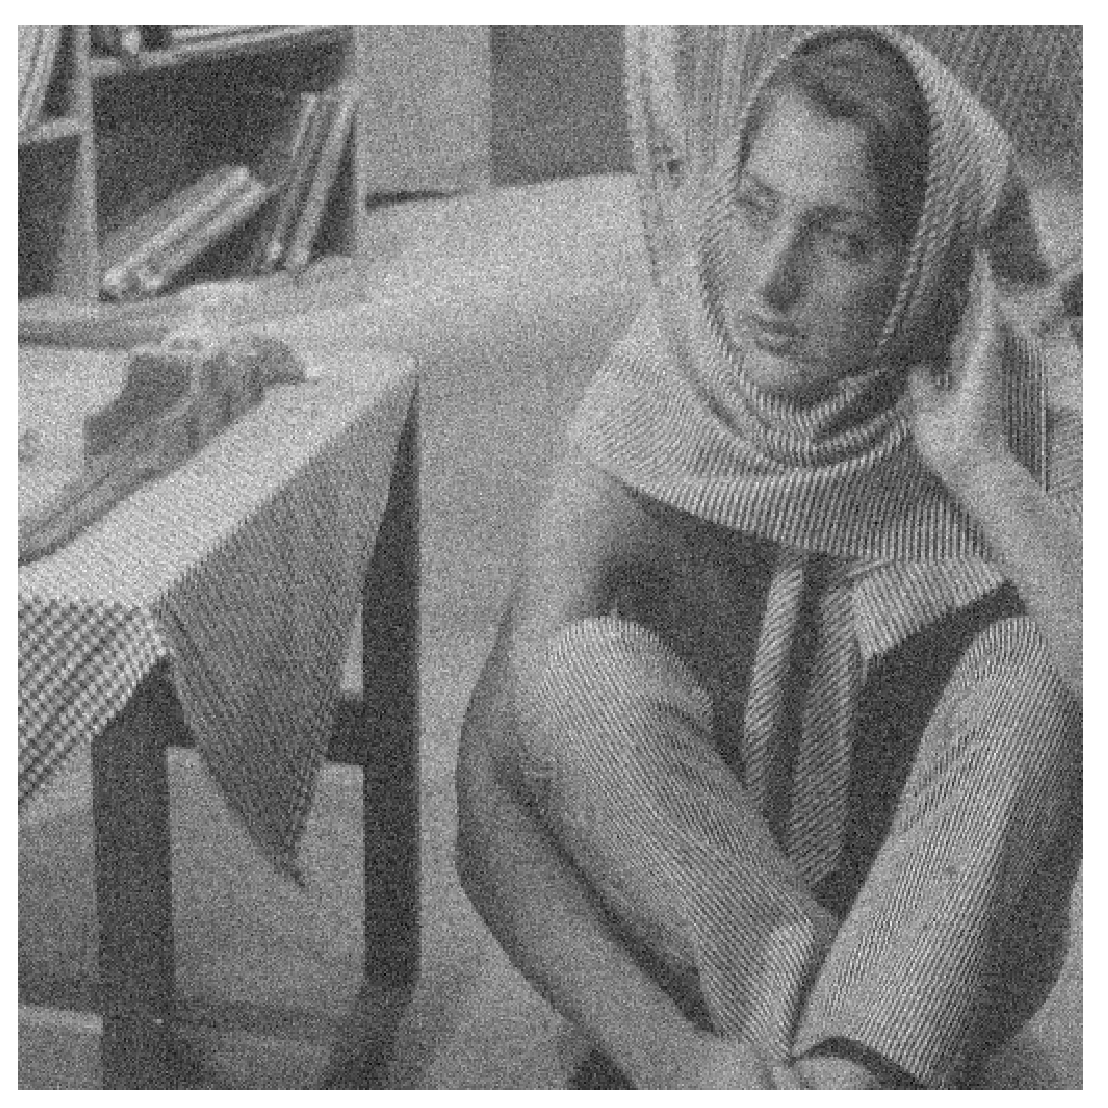
\includegraphics[width=3cm]{./figures/4_1_noise.eps} & 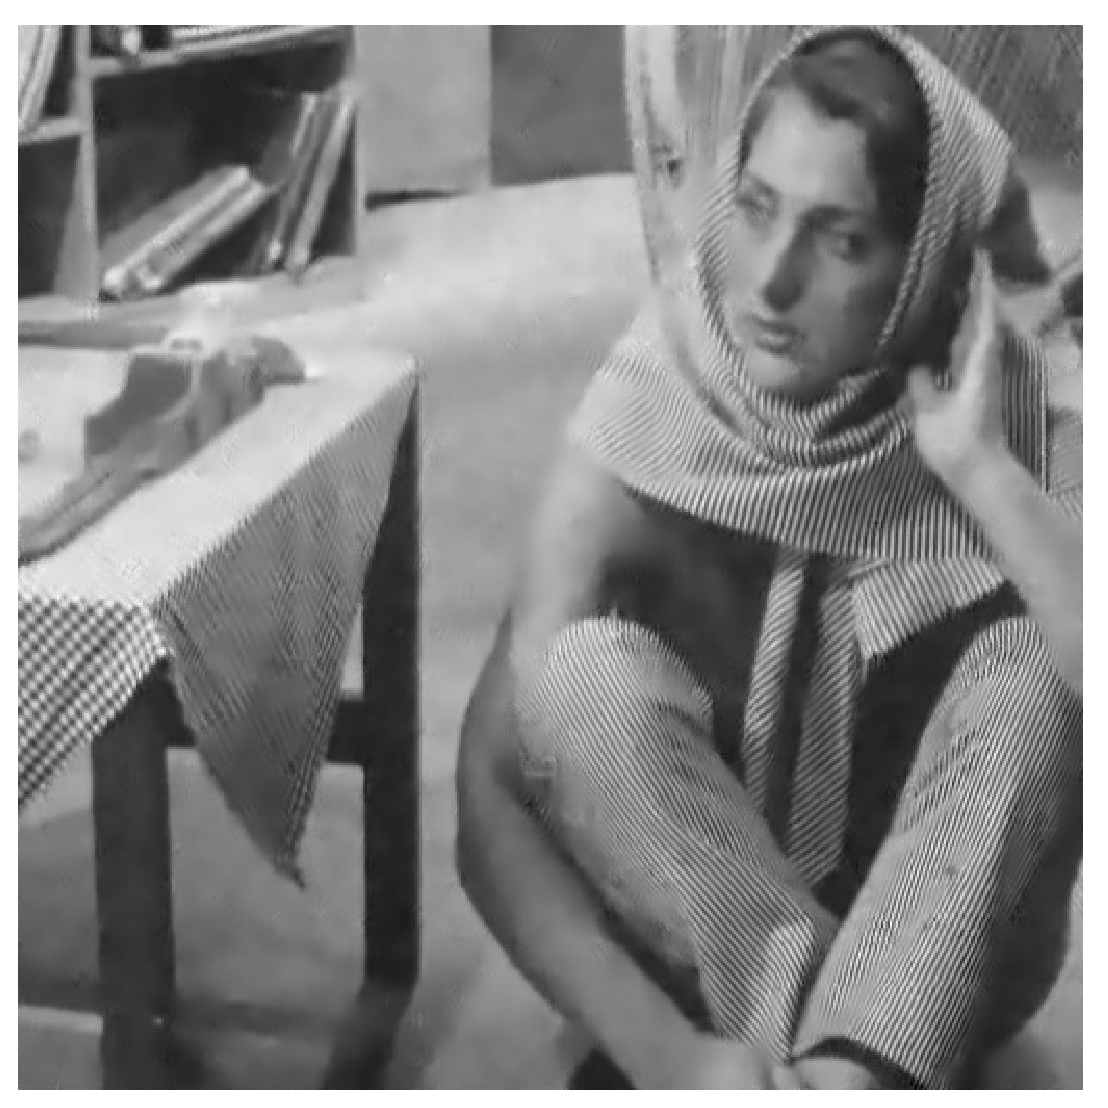
\includegraphics[width=3cm]{./figures/4_3_ksvd.eps}
&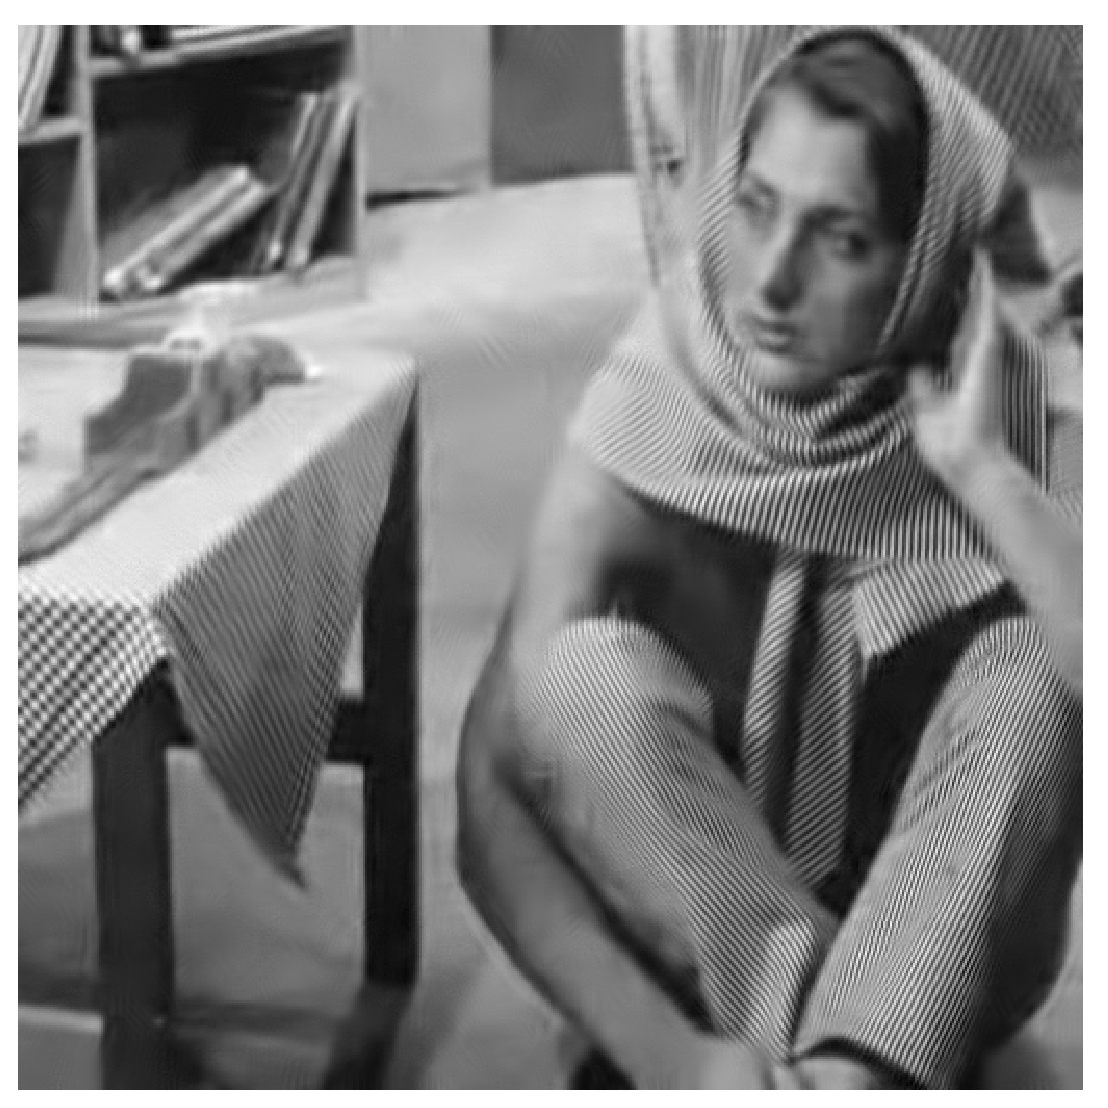
\includegraphics[width=3cm]{./figures/4_4_tfnoise.eps} & 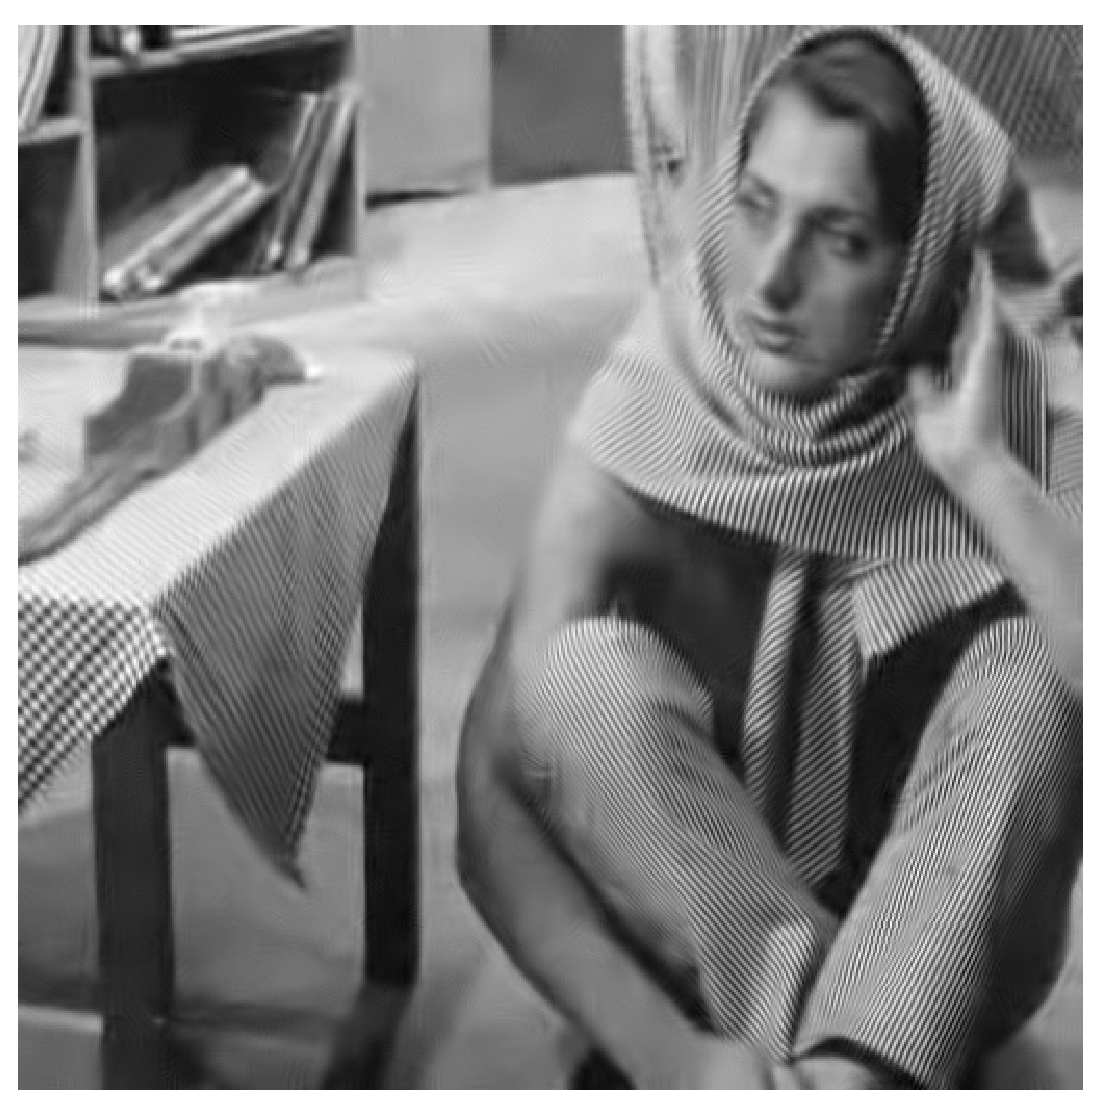
\includegraphics[width=3cm]{./figures/4_5_tfclean.eps}\\
 noisy image ($\sigma=0.1$)& k-svd(28.65dB) &TF noise(28.8dB) & TF clean(29.3dB) 
\end{tabular}
\end{center}

It seems the adaptive wavelet tight frames trained from clean is able to recover fine textures of the image, as shown in the images below.
\begin{center}
\begin{tabular}{c c c}
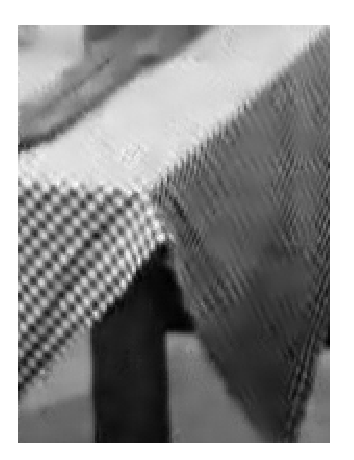
\includegraphics[width=3cm]{./figures/4_7.eps} & 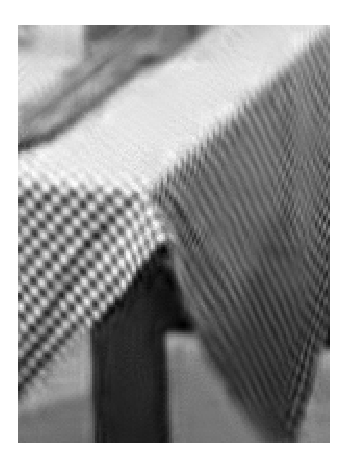
\includegraphics[width=3cm]{./figures/4_8.eps} &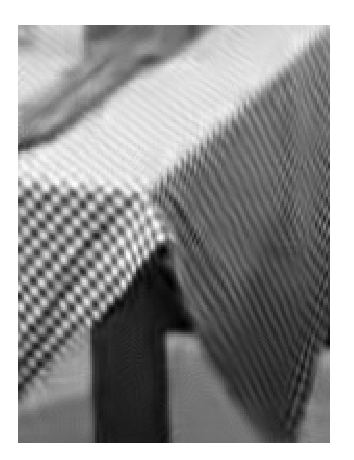
\includegraphics[width=3cm]{./figures/4_6.eps}\\
KSVD & TF noise & TF clean \\
\end{tabular}
\end{center}
There is a natural scenario where training filters from clean images makes sense such as in the second example, there is a dataset of human face images, some of them are corrupted by noise. We would like to train the filters from the clean images and apply them to the noisy images. We test this idea on the Yale human dataset B. A glimpse of the dataset is in Figure[]. We also add additive gaussian noise with $\sigma=0.1$. For filters learned form noisy images, the average PSNR is 31.35dB, for filters learned from clean images, the PSNR improves to 32.07dB, and for K-SVD the average PSNR is 31.4dB.
\begin{center}
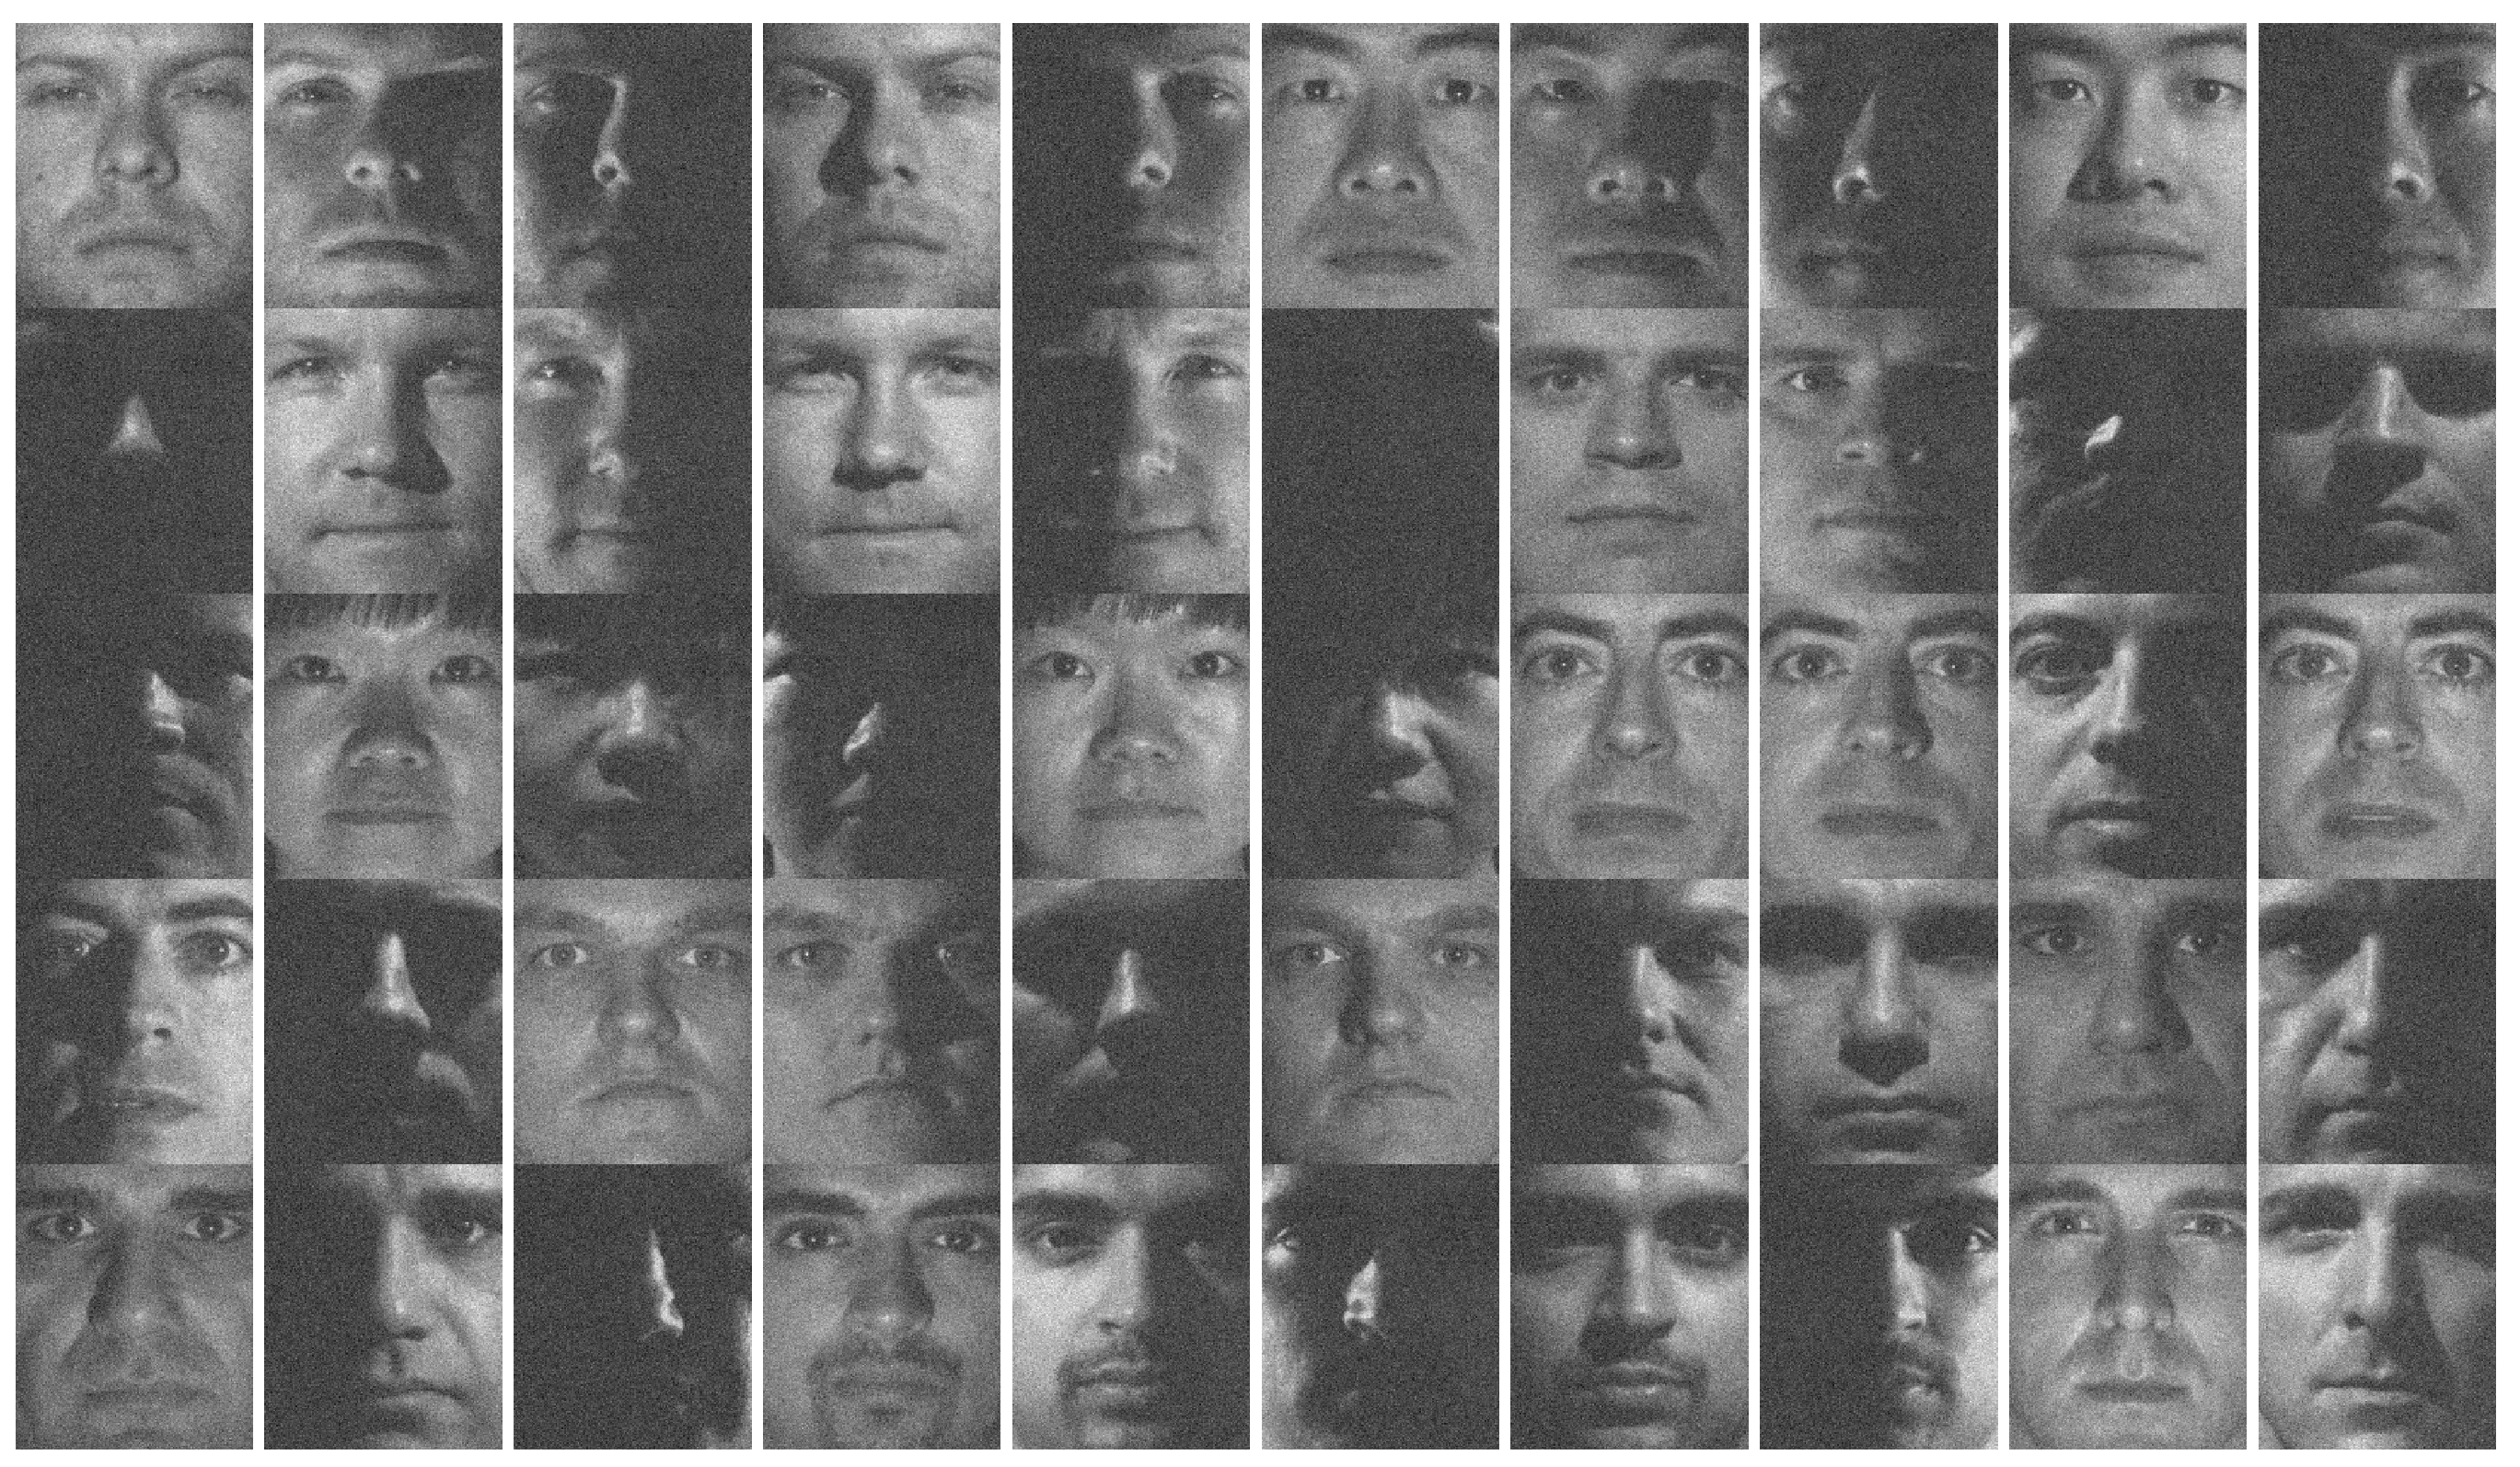
\includegraphics[width=6cm]{./figures/3_2.eps}
\end{center}
The third example is a natural image with unknown noise. Same as the previous two examples, we learn filters directly from the image. $\lambda$ is chosen to yield good visual. 

\begin{center}
\begin{tabular}{c c}
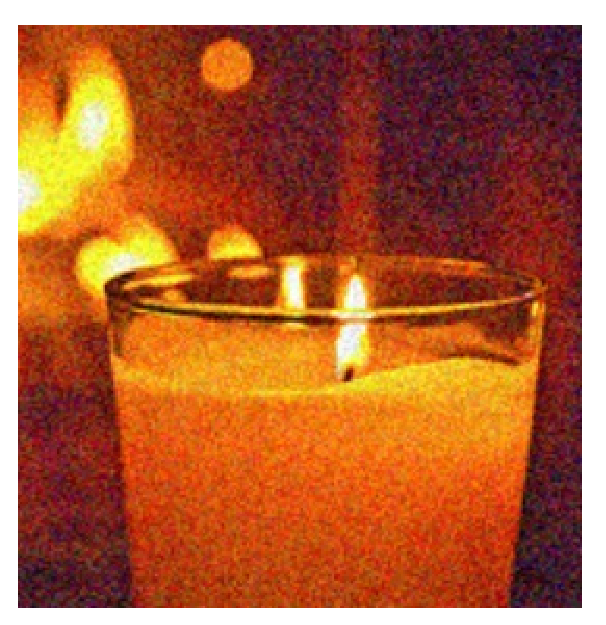
\includegraphics[width=4cm]{./figures/candle_noise.eps} & 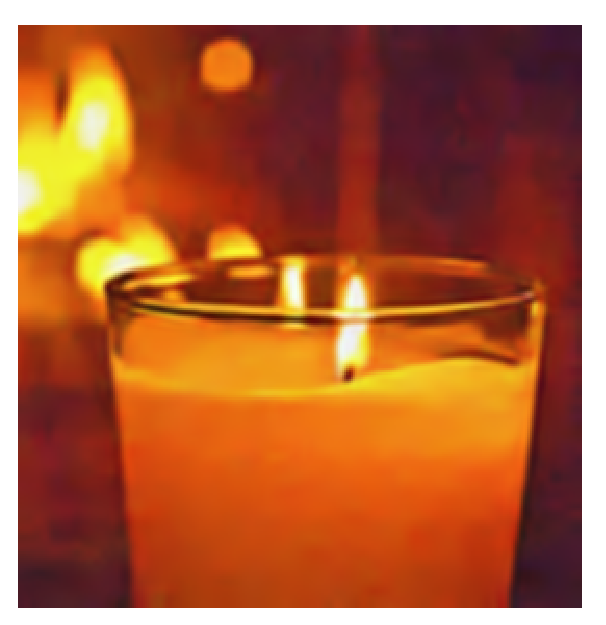
\includegraphics[width=4cm]{./figures/candle_clean.eps}\\
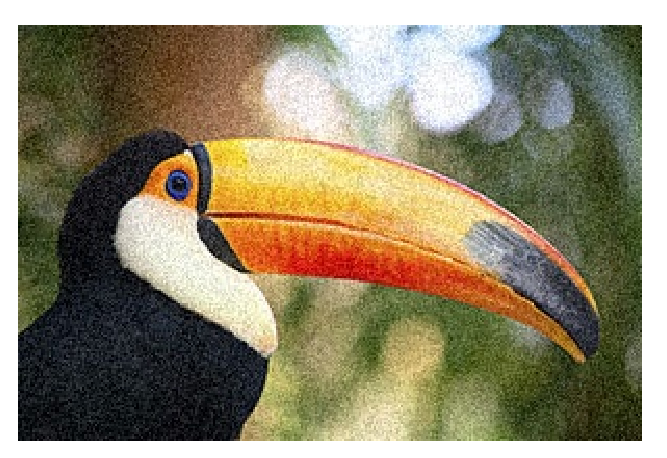
\includegraphics[width=4cm]{./figures/bird_noise.eps} & 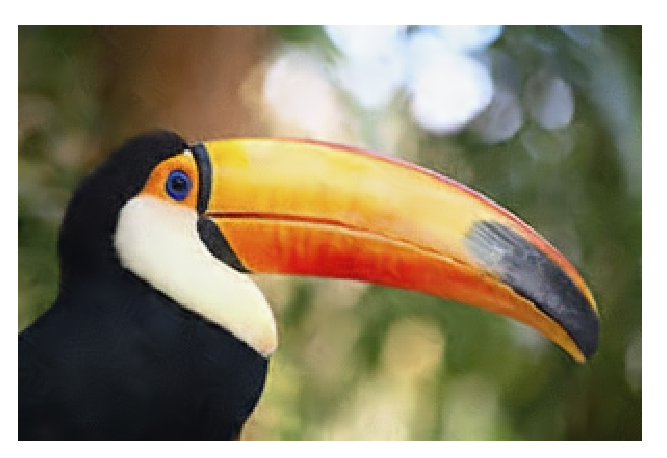
\includegraphics[width=4cm]{./figures/bird_clean.eps}\\
\end{tabular}
\end{center}

\subsection{classification}
In this experiment, we apply the representation obtained using the proposed model to examine its effectiveness on classification tasks. We choose to test on the MNIST handwritten digits dataest. It has 60000 training examples and 10000 test examples of digits 0-9. We adopt the third structure with two layers. Rectified linear activations are applied after the first layer. To do classification, we then send the output coefficients to a linear SVM.  Results with different number of filters are summarized in the following table.

As can be seen, there is a significant reduction in the error rates comapred to raw pixel features. State-of-the-art results are obtained using convolutional neural networks and virtual SVM, the best reported result without expanding the training set is 0.53\%.
\section{Discussions}
\subsection{Compare Dictionary Learning and Model A}
As we will see in this section, the dictionary learning models and model A share some similarities and have some differences. We make the following remarks: 

\textbf{1. Model A is convolutional form of dictionary learning.} Consider the training procedure of dictionary learning, given an image or a set of images, we collect all $r\times r$ non-overlapping patches and form them into a data matrix $X$, then we solve the following minimization program:
\begin{equation}
\min_{D,C} \|X-DC\|_2^2 + \lambda\|C\|_1.
\end{equation}
The underlying rationale is at some scale, say $r$, the image patch can be approximated by a sparse combination of some basis functions, where each column of $D$ represents a base function and each column of $C$ represents the combination coefficients for a particular patch.
Consider model A in the one layer case, the objective function is 
\begin{equation}
\label{eq2}
\min_{a_1,\cdots,a_m,v^{0}\cdots ,v^{m}} \|x-\sum_{i=1}^{m} a_i*v^{i}\|_2^2 +\lambda \sum_{i=1}^{m} \|v^{i}\|_1
\end{equation}
With some reorganization, this can be brought into a form that is very similar to dictionary learning. Let $X$ be the matrix formed by collecting all overlapping $r\times r$ images from an image, where each column of $X$ represents a vectorized image patch. Let $A=(vec(a_1),\cdots, vec(a_m))$, and $V$ is coefficient matrix which is reshaped conformally. Then the two terms in equation \eqref{eq2} are equivalent to :
\begin{equation}
\min_{A,V} \|X-AV\|_2^2+\lambda \|V\|_1.
\end{equation}
This is exactly the same form as dictionary learning except for that in dictionary learning, the $X$ is formed from non-overlapping patches while in model A, $X$ is formed from overlapping patches. If we accept the premise that image patches are translation invariant at a certain small scale, then convolutional models are a natural choice. In fact, for the purpose of finding local basis, we could form $X$ by sampling randomly uniformly from the image. It should not be hard to show when the sample size is large, the resulted basis converges to the one obtained by solving \eqref{eq2}. The way dictionary learning forms the matrix $X$ corresponds to uniform sampling from a special non-lapping grid, hence a proper subset of all $r\times r$ image patches, which is unnatural. There are subsequent works on dictionary learning forming matrix $X$ by collecting two or more sets of non-overlapping image patches, which is more close to the translation invariance assumption.

Despite the formal similarities, there are usually striking difference between the two models in practice. For example, In the practice of training dictionary learning models, people often use very large number of dictionary atoms(256 or more), where as in convolutional bases, we only use a small number of basis function(usually no more than 32). The patch based reconstruction results visually unpleasant block effect, which needs to be removed by post processing, while model A does not have such an issue.(But critically sampled model may or may not suffer from block effect depending on the support of the filter.)

\textbf{2. Model A generalizes to multiple layers}. Being able to generalize to multiple layers of transform is crucial to a multi-scale representation. However, dictionary learning, in its original form, cannot achieve this objective. In dictionary learning, a dictionary is obtained and each image patch is associated with a few combination coefficients. As these coefficients are unordered and are of different length for different image patches, there is no obvious way how to continue learning the pattern of the coefficients in a similar "dictionary learning" fashion. In comparison, in model A, the coefficients associated with the image are still placed on a regular grid, which, after downsampling, are still of the same format as the input, which facilitates further learning in almost the same way. It is exactly this feature that allows model A to operates on multiple scales. 

\textbf{3. Computationally, the analysis based variant is favorable to dictionary learning}. When the parameters of both models are trained and to be used for inference, the computational costs are different. To infer the codes of a new incoming signal, dictionary learning performs a sparse coding, common procedures include matching pursuit, orthogonal matching pursuit and some path following algorithms, and they are of  different computational complexity. To solve model A in the synthesis formulation would require the same computation. However, there is an analysis based variant of model, which is far more efficient computationally in that it requires only a convolution plus a point-wise operation( such as thresholding). Compared with algorithms for solving sparse coding, there is a dramatic performance gain.

\subsection{Connection with convoluvional neural network}
The analysis based multi-scale structure resembles the deep convolutional neural networks even though we starts from a very different perspective, the wavelet tight frames. Despite the structure similarity, there are some striking difference between them. First, the convolutional neural network is a purely supervised learning machine, while the proposed model is unsupervised. Second, the proposed model is constructed with respect to the unitary extension principle, hence has the nearly perfect reconstruction property, whereas in deep convolutional neural networks, it is not clear how to reconstruct the input as much information is lost as we ascend the layers. In other words, the proposed model is a nearly lossless decomposition of the input signal, while the neural network is not.
Studying the deeper connections between the analysis based multi-scale representations and the convolutional neural nets will be future direction.

\section{Conclusion}
In this paper, we proposed a novel model that serve as a multi-scale adaptive representations of image signals. This representation improves over dictionary learning in two ways: the first is encoding efficiency, and the second is a truly multi-scale architecture. Numerical illustrations are given to show the potential effectiveness of this new representation. In addition, the new representation has the property of being robust to translations and deformations. Interesting connections between the proposed model and dictionary learning as well as auto-encoders are established. We believe the proposed model can be an alternative to existing predefined wavelet tight frames and dictionary learning approach in some applications.
\section{Appendix}
\subsection{Numerical Algorithms}

The optimization program \eqref{model:m1} can be solved using interior-point method, but it is relatively slow for large problems. We also consider the following split Bregman algorithm, which is faster. The program we want to solve is 
\begin{equation}
\begin{aligned}
&\min_{a_1,\cdots,a_m} \sum_j \|v_j\|_1 \\
\textrm{subject to} \quad & v_j = a_j(-\cdot)*x \\
	& \{a_i\}_{i=1}^m \in \mathcal{C}.
	\end{aligned}
\end{equation}

The split Bregman algorithm for this program can be written in the following steps:
\begin{equation}
\label{breg:all}
\begin{aligned}
	(v^{k+1},a^{k+1}) &=\arg\min_{v,a} \sum_j \|v_j\|_1 + \lambda\sum_j\|a_j(-\cdot)*x+b_j^k-v_j\|_2^2 \quad\textrm{subject to} \quad \{a_i\}_{i=1}^m \in \mathcal{C}.\\
	b_j^{k+1} &= b_j^k + a_j^{k+1}(-\cdot)*x - v_j^{k+1} \\
\end{aligned}
\end{equation}

The first step can be subdivided into two steps:
\begin{equation}
\label{bregv}
		v^{k+1}  = \arg\min_{v_1,\cdots,v_m}  \sum_j \|v_j\|_1 + \tau \|a^k_j(-\cdot)*x +b^k_j -v_j\|_2^2
\end{equation}
\begin{equation}
\label{brega}
a^{k+1} =\arg\min_a \sum_j \|a_j(-\cdot)*x+b^{k}_j-v^{k+1}_j\|_2^2   \quad\textrm{subject to} \quad \{a_i\}_{i=1}^m \in \mathcal{C}.\\
\end{equation}

Now \eqref{bregv} is given explicitly by soft thresholding:
\begin{equation}
	v^{k+1}_j = \mathcal{T}(a^k_j(-\cdot)*x+b^k_j,\frac{1}{2\lambda})
\end{equation}
and \eqref{brega} can be solved using interior point method. It makes no sense to solve $a$ beyond the precision of the uncertainty of $b$, a handful iterations will work. If the low frequency constraint is explicitly incorporated, the interior point steps should also be changed accordingly. Updating $b$ is straightforward.

Solving \eqref{eq:m3} basically follow the same lines, except that updating $a$ and $u$ is an unconstrained program hence we can run a few steps of conjugate gradient or quasi-Newton iterations to get desired accuracy.










\bibliography{ref}
\bibliographystyle{plain}

\end{document}